\begin{frame}[fragile]{Visualização de update(3, -2)}

    \begin{figure}
        \centering

        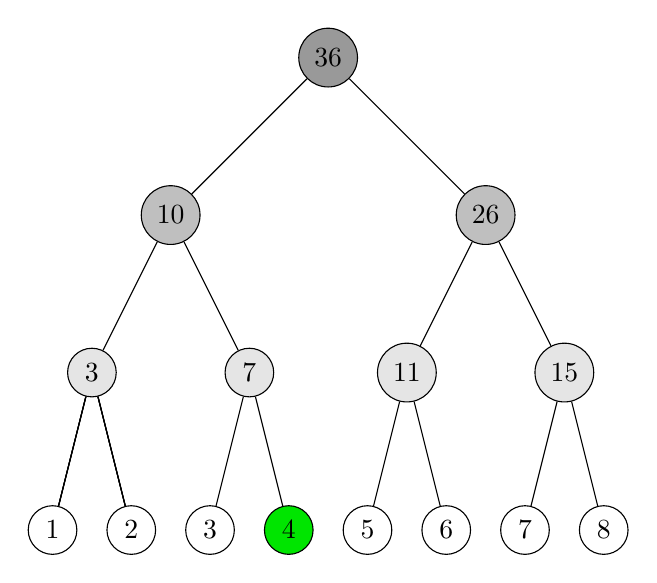
\begin{tikzpicture}
            \node[draw,circle] (A1) at (1, 0) { 1 };
            \node[draw,circle] (A2) at (2, 0) { 2 };
            \node[draw,circle] (A3) at (3, 0) { 3 };
            \node[draw,circle,fill=green!90!black] (A4) at (4, 0) { 4 };
            \node[draw,circle] (A5) at (5, 0) { 5 };
            \node[draw,circle] (A6) at (6, 0) { 6 };
            \node[draw,circle] (A7) at (7, 0) { 7 };
            \node[draw,circle] (A8) at (8, 0) { 8 };

            \node[draw,circle,fill=gray!20] (B1) at (1.5, 2) { 3 };
            \node[draw,circle,fill=gray!20] (B2) at (3.5, 2) { 7 };
            \node[draw,circle,fill=gray!20] (B3) at (5.5, 2) { 11 };
            \node[draw,circle,fill=gray!20] (B4) at (7.5, 2) { 15 };

            \node[draw,circle,fill=gray!50] (C1) at (2.5, 4) { 10 };
            \node[draw,circle,fill=gray!50] (C2) at (6.5, 4) { 26 };

            \node[draw,circle,fill=gray!80] (D1) at (4.5, 6) { 36 };

            \draw (A1) -- (B1);
            \draw (A2) -- (B1);
            \draw (A3) -- (B2);
            \draw (A4) -- (B2);
            \draw (A5) -- (B3);
            \draw (A6) -- (B3);
            \draw (A7) -- (B4);
            \draw (A8) -- (B4);
            \draw (A1) -- (B1);
            \draw (A2) -- (B1);
            \draw (A1) -- (B1);
            \draw (A2) -- (B1);
            \draw (A1) -- (B1);
            \draw (A2) -- (B1);
            \draw (B1) -- (C1);
            \draw (B2) -- (C1);
            \draw (B3) -- (C2);
            \draw (B4) -- (C2);
            \draw (C1) -- (D1);
            \draw (C2) -- (D1);
        \end{tikzpicture}
    \end{figure}

\end{frame}

\begin{frame}[fragile]{Visualização de update(3, -2)}

    \begin{figure}
        \centering

        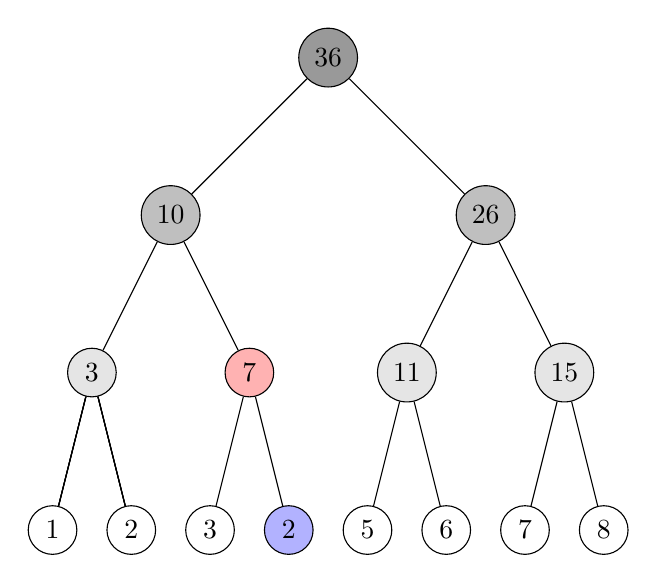
\begin{tikzpicture}
            \node[draw,circle] (A1) at (1, 0) { 1 };
            \node[draw,circle] (A2) at (2, 0) { 2 };
            \node[draw,circle] (A3) at (3, 0) { 3 };
            \node[draw,circle,fill=blue!30] (A4) at (4, 0) { 2 };
            \node[draw,circle] (A5) at (5, 0) { 5 };
            \node[draw,circle] (A6) at (6, 0) { 6 };
            \node[draw,circle] (A7) at (7, 0) { 7 };
            \node[draw,circle] (A8) at (8, 0) { 8 };

            \node[draw,circle,fill=gray!20] (B1) at (1.5, 2) { 3 };
            \node[draw,circle,fill=red!30] (B2) at (3.5, 2) { 7 };
            \node[draw,circle,fill=gray!20] (B3) at (5.5, 2) { 11 };
            \node[draw,circle,fill=gray!20] (B4) at (7.5, 2) { 15 };

            \node[draw,circle,fill=gray!50] (C1) at (2.5, 4) { 10 };
            \node[draw,circle,fill=gray!50] (C2) at (6.5, 4) { 26 };

            \node[draw,circle,fill=gray!80] (D1) at (4.5, 6) { 36 };

            \draw (A1) -- (B1);
            \draw (A2) -- (B1);
            \draw (A3) -- (B2);
            \draw (A4) -- (B2);
            \draw (A5) -- (B3);
            \draw (A6) -- (B3);
            \draw (A7) -- (B4);
            \draw (A8) -- (B4);
            \draw (A1) -- (B1);
            \draw (A2) -- (B1);
            \draw (A1) -- (B1);
            \draw (A2) -- (B1);
            \draw (A1) -- (B1);
            \draw (A2) -- (B1);
            \draw (B1) -- (C1);
            \draw (B2) -- (C1);
            \draw (B3) -- (C2);
            \draw (B4) -- (C2);
            \draw (C1) -- (D1);
            \draw (C2) -- (D1);
        \end{tikzpicture}
    \end{figure}

\end{frame}

\begin{frame}[fragile]{Visualização de update(3, -2)}

    \begin{figure}
        \centering

        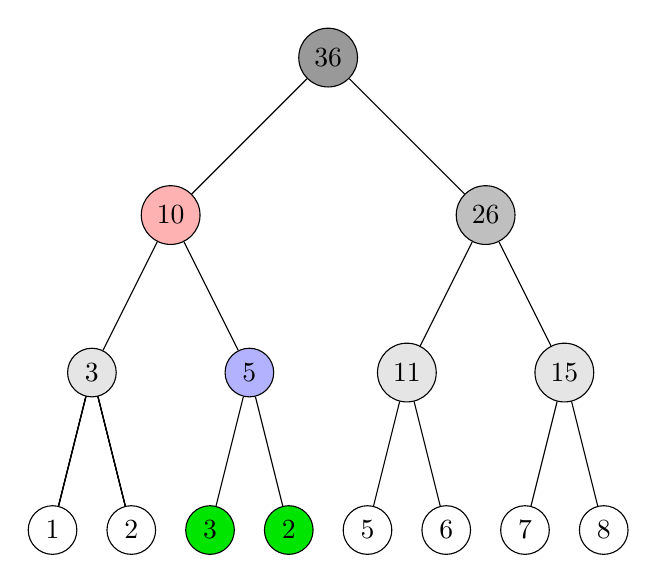
\begin{tikzpicture}
            \node[draw,circle] (A1) at (1, 0) { 1 };
            \node[draw,circle] (A2) at (2, 0) { 2 };
            \node[draw,circle,fill=green!90!black] (A3) at (3, 0) { 3 };
            \node[draw,circle,fill=green!90!black] (A4) at (4, 0) { 2 };
            \node[draw,circle] (A5) at (5, 0) { 5 };
            \node[draw,circle] (A6) at (6, 0) { 6 };
            \node[draw,circle] (A7) at (7, 0) { 7 };
            \node[draw,circle] (A8) at (8, 0) { 8 };

            \node[draw,circle,fill=gray!20] (B1) at (1.5, 2) { 3 };
            \node[draw,circle,fill=blue!30] (B2) at (3.5, 2) { 5 };
            \node[draw,circle,fill=gray!20] (B3) at (5.5, 2) { 11 };
            \node[draw,circle,fill=gray!20] (B4) at (7.5, 2) { 15 };

            \node[draw,circle,fill=red!30] (C1) at (2.5, 4) { 10 };
            \node[draw,circle,fill=gray!50] (C2) at (6.5, 4) { 26 };

            \node[draw,circle,fill=gray!80] (D1) at (4.5, 6) { 36 };

            \draw (A1) -- (B1);
            \draw (A2) -- (B1);
            \draw (A3) -- (B2);
            \draw (A4) -- (B2);
            \draw (A5) -- (B3);
            \draw (A6) -- (B3);
            \draw (A7) -- (B4);
            \draw (A8) -- (B4);
            \draw (A1) -- (B1);
            \draw (A2) -- (B1);
            \draw (A1) -- (B1);
            \draw (A2) -- (B1);
            \draw (A1) -- (B1);
            \draw (A2) -- (B1);
            \draw (B1) -- (C1);
            \draw (B2) -- (C1);
            \draw (B3) -- (C2);
            \draw (B4) -- (C2);
            \draw (C1) -- (D1);
            \draw (C2) -- (D1);
        \end{tikzpicture}
    \end{figure}

\end{frame}

\begin{frame}[fragile]{Visualização de update(3, -2)}

    \begin{figure}
        \centering

        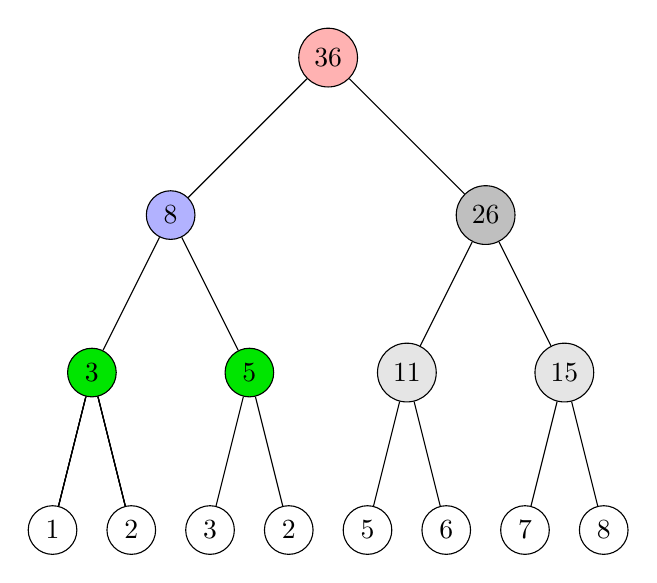
\begin{tikzpicture}
            \node[draw,circle] (A1) at (1, 0) { 1 };
            \node[draw,circle] (A2) at (2, 0) { 2 };
            \node[draw,circle] (A3) at (3, 0) { 3 };
            \node[draw,circle] (A4) at (4, 0) { 2 };
            \node[draw,circle] (A5) at (5, 0) { 5 };
            \node[draw,circle] (A6) at (6, 0) { 6 };
            \node[draw,circle] (A7) at (7, 0) { 7 };
            \node[draw,circle] (A8) at (8, 0) { 8 };

            \node[draw,circle,fill=green!90!black] (B1) at (1.5, 2) { 3 };
            \node[draw,circle,fill=green!90!black] (B2) at (3.5, 2) { 5 };
            \node[draw,circle,fill=gray!20] (B3) at (5.5, 2) { 11 };
            \node[draw,circle,fill=gray!20] (B4) at (7.5, 2) { 15 };

            \node[draw,circle,fill=blue!30] (C1) at (2.5, 4) { 8 };
            \node[draw,circle,fill=gray!50] (C2) at (6.5, 4) { 26 };

            \node[draw,circle,fill=red!30] (D1) at (4.5, 6) { 36 };

            \draw (A1) -- (B1);
            \draw (A2) -- (B1);
            \draw (A3) -- (B2);
            \draw (A4) -- (B2);
            \draw (A5) -- (B3);
            \draw (A6) -- (B3);
            \draw (A7) -- (B4);
            \draw (A8) -- (B4);
            \draw (A1) -- (B1);
            \draw (A2) -- (B1);
            \draw (A1) -- (B1);
            \draw (A2) -- (B1);
            \draw (A1) -- (B1);
            \draw (A2) -- (B1);
            \draw (B1) -- (C1);
            \draw (B2) -- (C1);
            \draw (B3) -- (C2);
            \draw (B4) -- (C2);
            \draw (C1) -- (D1);
            \draw (C2) -- (D1);
        \end{tikzpicture}
    \end{figure}

\end{frame}

\begin{frame}[fragile]{Visualização de update(3, -2)}

    \begin{figure}
        \centering

        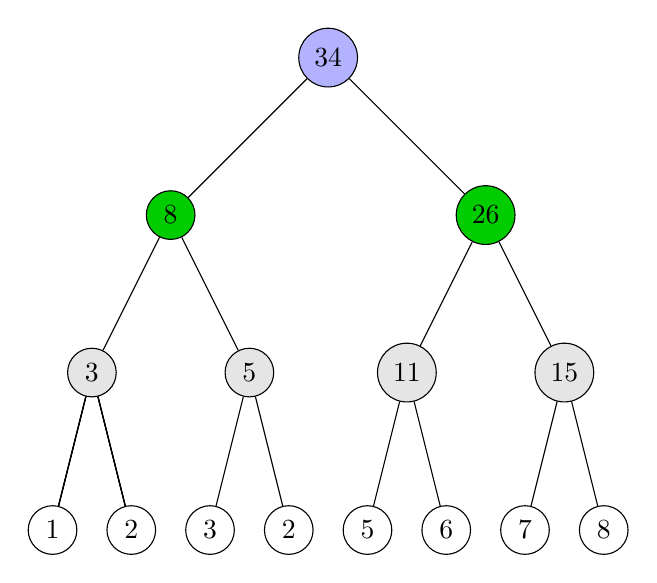
\begin{tikzpicture}
            \node[draw,circle] (A1) at (1, 0) { 1 };
            \node[draw,circle] (A2) at (2, 0) { 2 };
            \node[draw,circle] (A3) at (3, 0) { 3 };
            \node[draw,circle] (A4) at (4, 0) { 2 };
            \node[draw,circle] (A5) at (5, 0) { 5 };
            \node[draw,circle] (A6) at (6, 0) { 6 };
            \node[draw,circle] (A7) at (7, 0) { 7 };
            \node[draw,circle] (A8) at (8, 0) { 8 };

            \node[draw,circle,fill=gray!20] (B1) at (1.5, 2) { 3 };
            \node[draw,circle,fill=gray!20] (B2) at (3.5, 2) { 5 };
            \node[draw,circle,fill=gray!20] (B3) at (5.5, 2) { 11 };
            \node[draw,circle,fill=gray!20] (B4) at (7.5, 2) { 15 };

            \node[draw,circle,fill=green!80!black] (C1) at (2.5, 4) { 8 };
            \node[draw,circle,fill=green!80!black] (C2) at (6.5, 4) { 26 };

            \node[draw,circle,fill=blue!30] (D1) at (4.5, 6) { 34 };

            \draw (A1) -- (B1);
            \draw (A2) -- (B1);
            \draw (A3) -- (B2);
            \draw (A4) -- (B2);
            \draw (A5) -- (B3);
            \draw (A6) -- (B3);
            \draw (A7) -- (B4);
            \draw (A8) -- (B4);
            \draw (A1) -- (B1);
            \draw (A2) -- (B1);
            \draw (A1) -- (B1);
            \draw (A2) -- (B1);
            \draw (A1) -- (B1);
            \draw (A2) -- (B1);
            \draw (B1) -- (C1);
            \draw (B2) -- (C1);
            \draw (B3) -- (C2);
            \draw (B4) -- (C2);
            \draw (C1) -- (D1);
            \draw (C2) -- (D1);
        \end{tikzpicture}
    \end{figure}

\end{frame}
